
\chapter{Using Convolutional Neural Networks to separate ${\mu}'s$ from ${\pi}'s$}


The work shown in these next sections are based on the previous work done described in \cite{priorwork}. That CNN (now referred to as CNN1075) was trained using single generated isotropic muons and pions from 0-2 GeV energy range. 1,075 muons and pions were used to train the network and 1,075 $\mu/\pi$ were used as a validation set. The accuracy is how well CNN1075 is doing by epoch and was 74.5\%. The loss is gradient descent or minimization of the error of the weights and biases used in each neuron of each layer of CNN1075 and was 58\% with a trend sloping downwards on the loss curve as well as a trend sloping upward in the accuracy curve. Due to the depth of the neural network framework, it was necessary to train with a larger dataset and for more epochs, however, the downward slope of the loss curve is an indication that once trained for longer with a higher training sample, neural networks can be used for $\mu/\pi$ separation. Updates in the image making and downsampling algorithm were made to fix issues that arose in CNN1075. 

\section{Image Making Scheme}\label{image_making} 

The $\mu/\pi$ image dataset used to train and test the second CNN (now referred to as CNN10000) was created using single generated isotropic muons and pions from 0-2 GeV energ range. 10,000 muons and 10,000 pions were used for training and testing split 50\%. The images were created based on wire number and time tick in the collection plane. Uboonecode v06{\_}23{\_}00 was used instead of v05{\_}08{\_}00 which was used previously. The wire signal was the raw ADC value after noise filtering. Each collection plane grayscale image was 3456x1280x1 where 5 time ticks were pooled into 1 bin which is different than the previous dataset and was implemented due to the fact that the time ticks of an event went from 9400 to 6400 with the change of uboonecode version. The grayscale color standard is 8bit therefore the ADC value of wire and time tick was also downsampled due to the 12bit ADC value MicroBooNE has. To do this, the highest ADC pixel in the image was found and then this was divided by the rest placing all pixel values between 0-1. From there, all pixel values are then multiplied by 255. All images were made using a LArSoft module. Once the images were created, using and image manipulation framework called OpenCV images were read into a numpy array and cropped to the region of interest by only keeping rows and columns where all ADC values are higher than 0 and then resized it to 224x224 using OpenCV's resize function. This downsampling of ADC values creates a problem of information loss for example, a proton which is highly ionizing will have the same brightness as a minimum ionizing muon by virtue of how the images are created. Creating images that thoroughly depict the ADC scale for use in $dE/dx$ particle identification has been implemented and retraining of CNN is underway.
Issues that arose in CNN1075 that were fixed in CNN10000 include zero-padding images in X and Y that are smaller than 224X224 to eliminate over-zooming effect and fixing a bug that shifted pixels separated by a dead-wire region. 

Images were also made from events that passed the cc-inclusive selection 1 filter right before the 75 cm track length cut and were classified using the CNN10000. The dataset used to create these images is the same one used in \cite{cc-inclusive}, prodgenie{\_}bnb{\_}nu{\_}cosmic{\_}uboone{\_}mcc7{\_}reco2. These images were created using information from the track candidate that passed the filter. Only wire number and time ticks associated to the track candidate were drawn on the image to mimic a single particle generated image. These images were then classified using CNN10000. Two approaches were taken in making these images. The first was using the image normalization above where the maximum pixel in each image is used as a normalization constant to get all pixels between 0-1 then multiply all pixels by 255. As described above, this is the incorrect way to normalize; it should be normalized by dataset not by event, which is the second way the images were created. The results of CNN10000 performance are shown in section \ref{research approach}. 


\section{Convolutional Neural Network Training}\label{research approach}
The hyperparameters used for CNN10000 are shown. The batch size for the training and testing as well as the test iter were chosen to encompass the whole training/testing image set when doing accuracy/loss calculations. To do this, multiplying the test iter by the test batch size give you the amount of images used when calculating accuracy/loss curves. For reference, the accuracy and loss are defined as well. 


\begin{itemize}
 \item \verb|train_batch_size: 100|
 \item \verb|test_batch_size: 100|
 \item \verb|test_iter: 100|
 \item \verb|test_interval: 100|
 \item \verb|base_lr: 0.001|
 \item \verb|lr_policy: "step"|
 \item \verb|gamma: 0.1|
 \item \verb|stepsize: 1000|
 \item \verb|display: 100|
 \item \verb|max_iter: 10000|
 \item \verb|momentum: 0.99|
 \item \verb|weight_decay: 0.0005|
 \item \verb|snapshot: 100|
\item Accuracy: How often the CNN predicts the truth over total number of images
\item Loss: Error between truth and prediction. Minimize loss by gradient descent to update weights and biases of CNN
\end{itemize}

The same architecure that was used to train CNN1075 was employed on CNN10000, Imagenet. Caffe \cite{caffe} was the software package used for both CNNs. The differences include batch size and test{\_}iter and momentum to account for the larger dataset. Both CNNs were trained on a CPU machine, Syracuse01. Further training will be done on a GPU cluster stationed at Syracuse University. Figure \ref{fig:loss_accuracy} shows the loss and accuracy of CNN10000. There is around a 10\% increase in accuracy from CNN1075 to CNN10000, 85\%, and around a 20\% decrease in loss, 36\%.      

\begin{figure}[htp!]
\centering
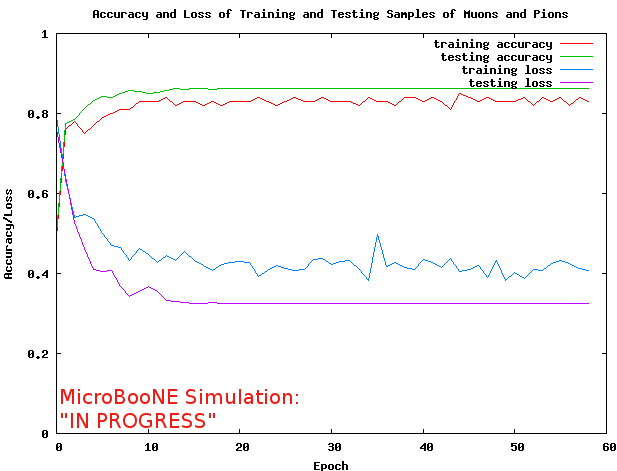
\includegraphics[scale=.55]{figs/acc_loss_10000_062117.png}
\caption{Accuracy vs. Loss of ImageNet 2-output $\mu/\pi$ sample consisting of ~10000 images each.} 
\label{fig:loss_accuracy}
\end{figure}

\begin{figure}[htp!]
\centering
	\begin{subfigure}[b]{.4\textwidth}
	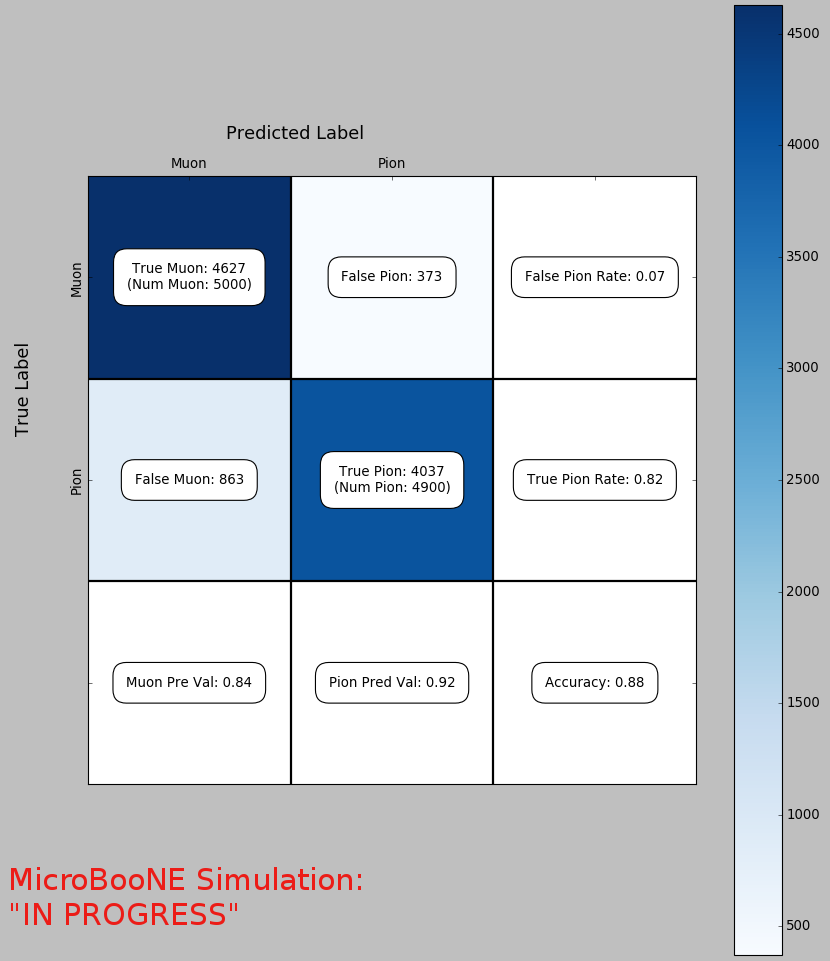
\includegraphics[width=\textwidth,height=3in]{figs/train_confusion-9-14-16.png}
	\caption{Confusion Matrix showing Accuracy of CNN using training data}
	\label{fig:confusion}
	\end{subfigure}
	\quad
	\begin{subfigure}[b]{.4\textwidth}
	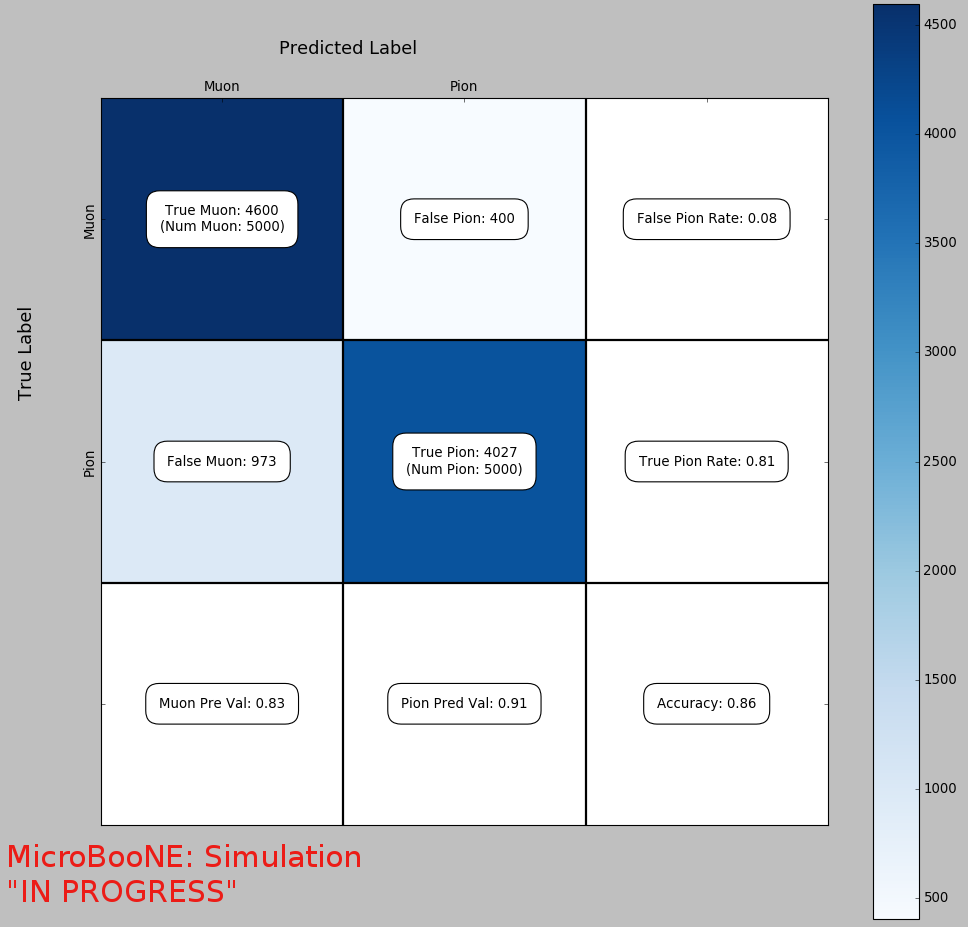
\includegraphics[width=\textwidth,height=3in]{figs/val_confusion_9-14-16.png}
	\caption{Confusion Matrix showing Accuracy of CNN using testing data}
	\label{fig:confusion_test}
	\end{subfigure}
	\quad
	\begin{subfigure}[b]{\textwidth}
	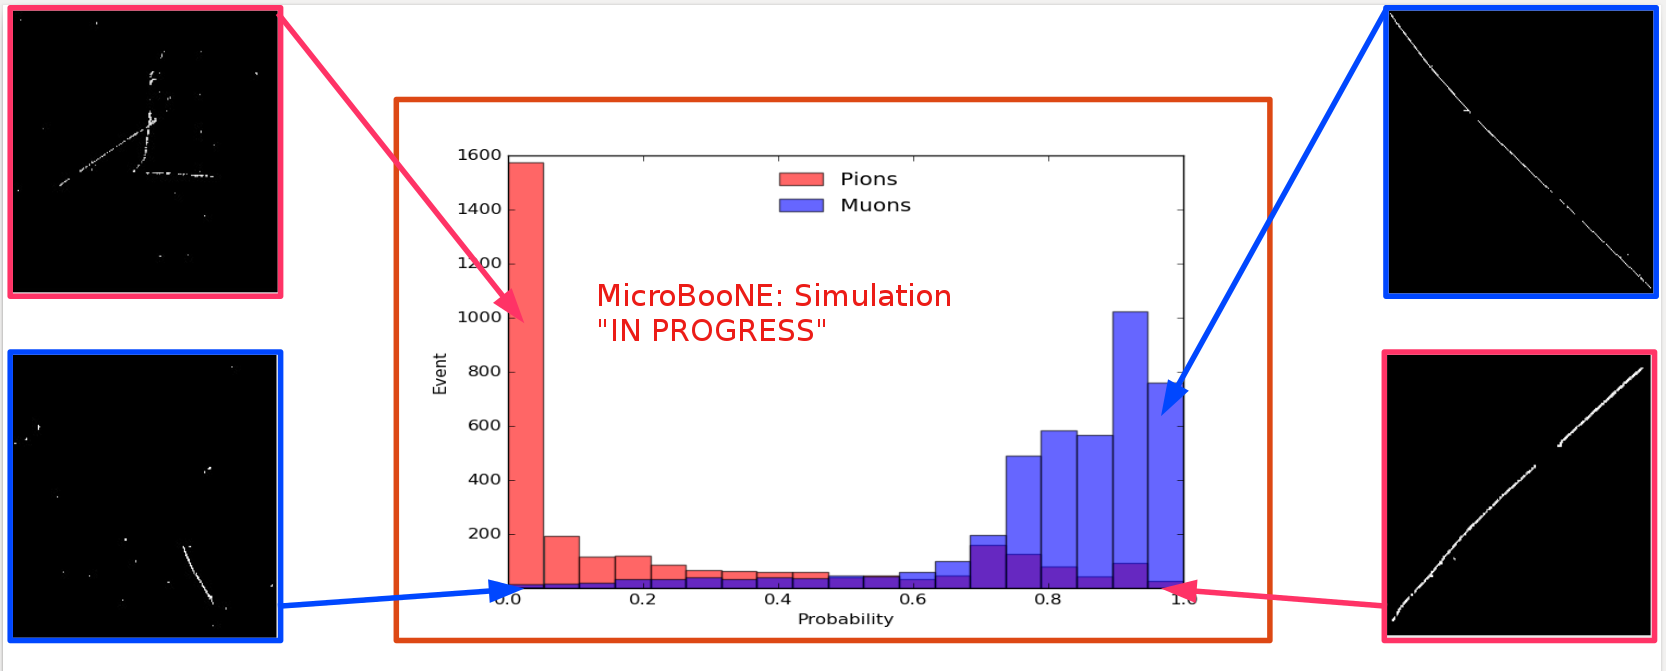
\includegraphics[width=\textwidth,height=2.5in]{figs/mitch_hw.png}
	\caption{Probability plot of muons and pions from testing set. Images surrounding histogram are a random event from lowest bin and highest bin for each particle.}
	\label{fig:prob_plot}
	\end{subfigure}
\caption{Description of confusion matrix varables: False pion rate = $false \pi/ total \pi$ True pion rate = $true \pi/total \pi$ Accuracy = $(true \pi rate + true \mu rate)/2$ Pion prediction value = $true \pi/(true \pi + false \pi)$ Muon prediction value = $true \mu/(true \mu + false \mu)$ \ref{fig:prob_plot} The probability plot includes muons and pions that are classified as primary particles.}
\label{fig:CNN_train}
\end{figure}

Figure \ref{fig:CNN_train} show a breakdown of $\mu/\pi$ separation for CNN10000. It also shows the network is not being overtrained due to the Accuracy of both the training and testing datasets being within .01\% of eachother. The CNN is doing a very good job of classifying true muons as muons, and our loss increase from CNN1075 is due to the increase in accuratly classifing pions as pions. 


%\begin{figure}[htp]
%\centering
%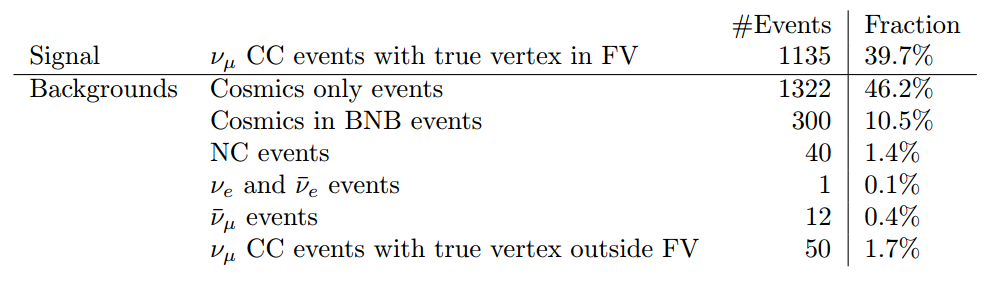
\includegraphics[width=.9\linewidth]{Purity_numbers.png}
%\caption{ Signal and background event numbers at final selection level estimated from a BNB+Cosmic sample and Cosmic only sample normalized to $5*10^{19}$ POT. The last column gives the fraction of this signal or background type to the total 2604 selected events.} 
%\label{fig:puritytable}
%\end{figure}

\section{Classification of MC data using Selection I Original CC-Inclusive Filter}\label{sel1orig}

\begin{figure}[htp!]
\centering
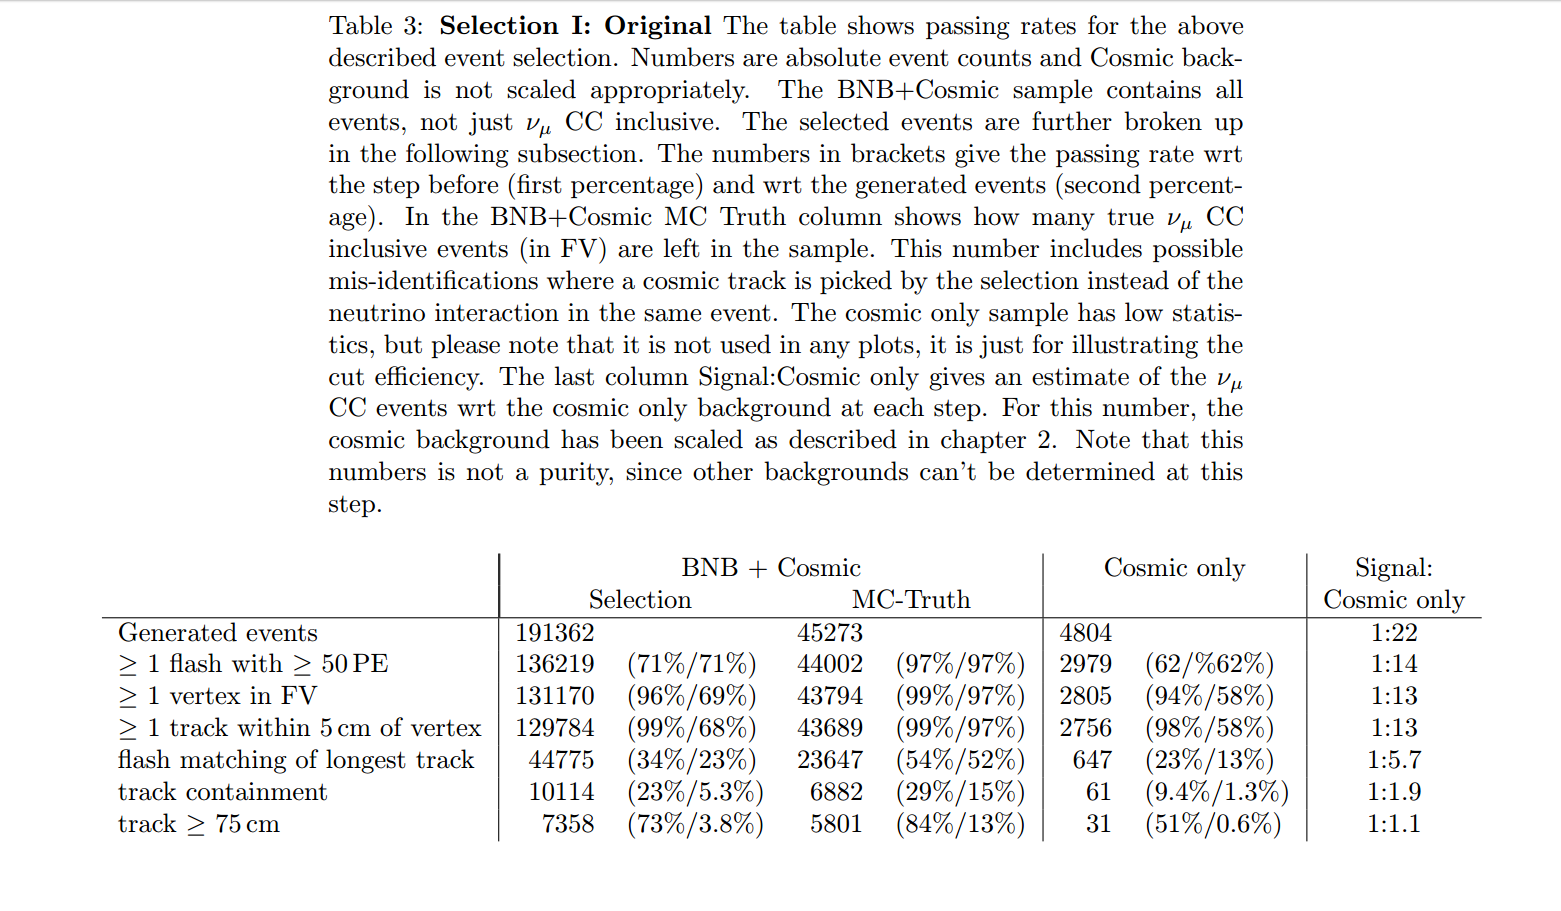
\includegraphics[width=.9\textwidth]{figs/sel1_cuts.png}
\caption{Snapshot of passing rates of Selection I from CC-Inclusive Filter} 
\label{fig:cuttable}
\end{figure}

\begin{figure}[htp!]
\centering
	\begin{subfigure}[b]{.45\textwidth}
	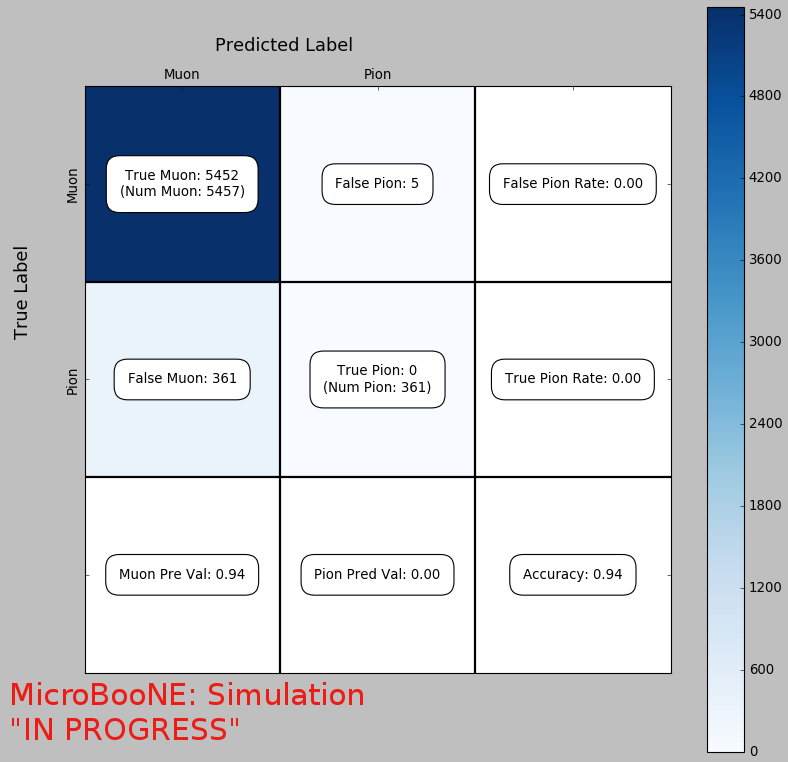
\includegraphics[width=3in,height=3in]{figs/confusion_0621_wrongnorm.png}
	\caption{Confusion Matrix showing Accuracy of CNN using data with wrong normilazion}
	\label{fig:confusion_wrongnorm}
	\end{subfigure}
	\quad
	\begin{subfigure}[b]{.45\textwidth}
	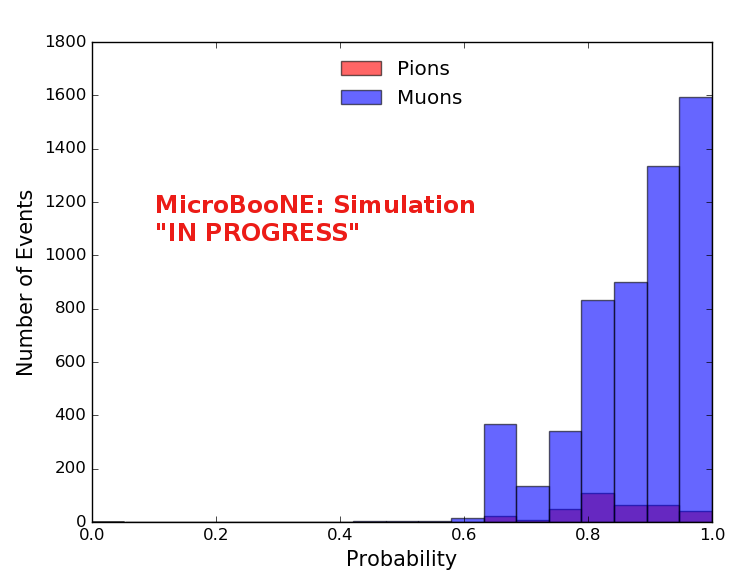
\includegraphics[width=3in,height=3in]{figs/prob_0706_wrongnorm_sel1.png}
	\caption{Probability plot showing $\mu/\pi$ separation of CNN using wrong normalization}
	\label{fig:prob_wrongnorm}
	\end{subfigure}
	\quad
	\begin{subfigure}[b]{.45\textwidth}
	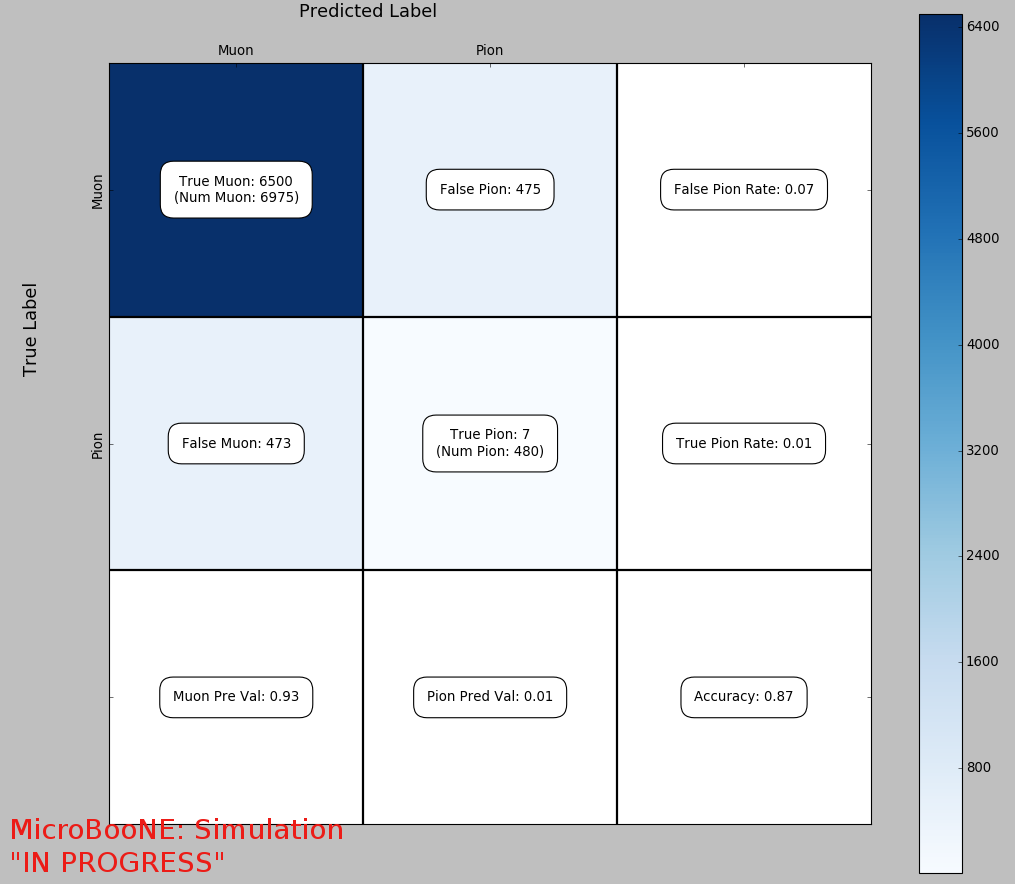
\includegraphics[width=3in,height=3in]{figs/confusion_rightnorm_0621.png}
	\caption{Confusion Matrix showing Accuracy of CNN using data with correct normilazion}
	\label{fig:confusion_rightnorm}
	\end{subfigure}
	\quad
	\begin{subfigure}[b]{.45\textwidth}
	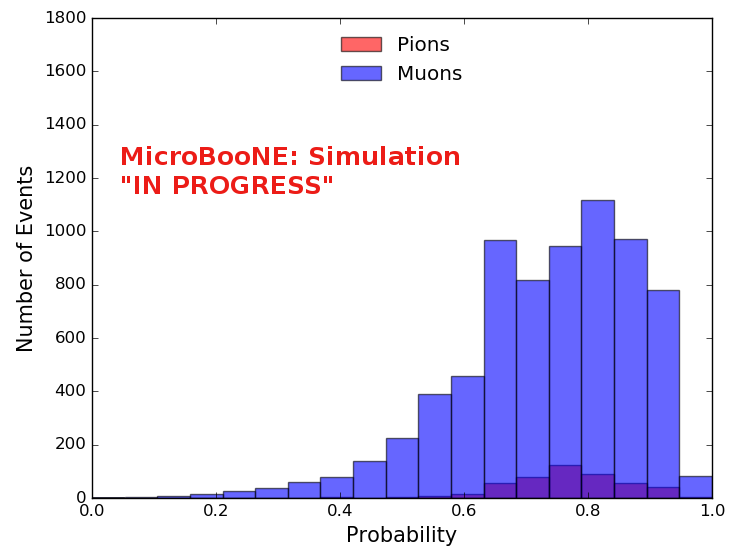
\includegraphics[width=3in,height=3in]{figs/prob_0706_rightnorm_sel1.png}
	\caption{Probability plot showing $\mu/\pi$ separation of CNN using correct normalization}
	\label{fig:prob_rightnorm}
	\end{subfigure}
	\quad
\caption{Results of CNN10000 classification of track candidate images output from cc-inclusive filter.}
\label{fig:CNN_ccnc}
\end{figure}

\begin{figure}[htp!]
\centering
	\begin{subfigure}[b]{.45\textwidth}
	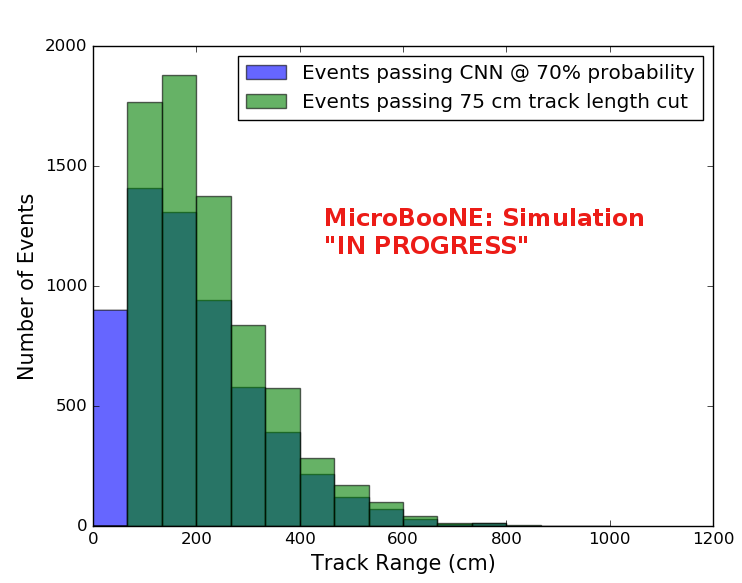
\includegraphics[width=3in,height=3in]{figs/sel1_trackrange_wrongnorm_acc70_0706.png}
	\caption{Track range distribution of events from Selection I Original passing CNN with 70\% accuracy using image data with wrong normilazion}
	\label{fig:track_wrongnorm}
	\end{subfigure}
	\quad
	\begin{subfigure}[b]{.45\textwidth}
	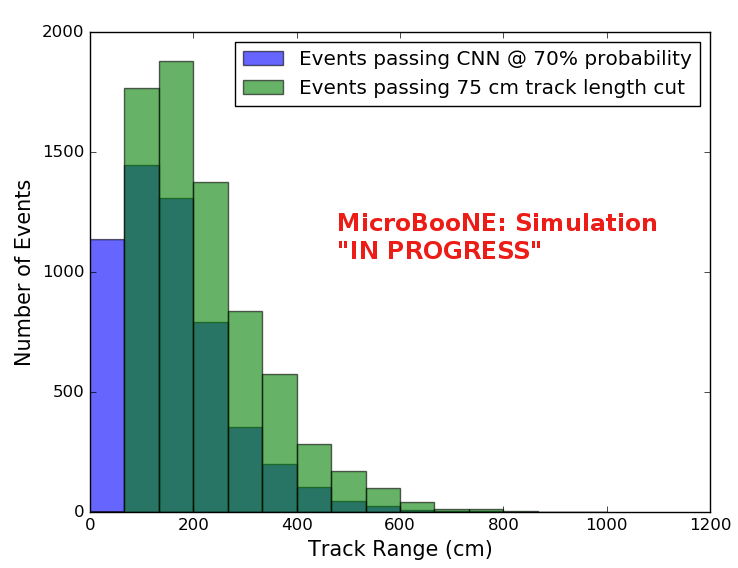
\includegraphics[width=3in,height=3in]{figs/sel1_trackrange_rightnorm_acc70_0706.png}
	\caption{Track range distribution of events from Selection I Original passing CNN with 70\% accuracy using image data with correct normilazion}
	\label{fig:track_rightnorm}
	\end{subfigure}
	\quad
	\begin{subfigure}[b]{.45\textwidth}
	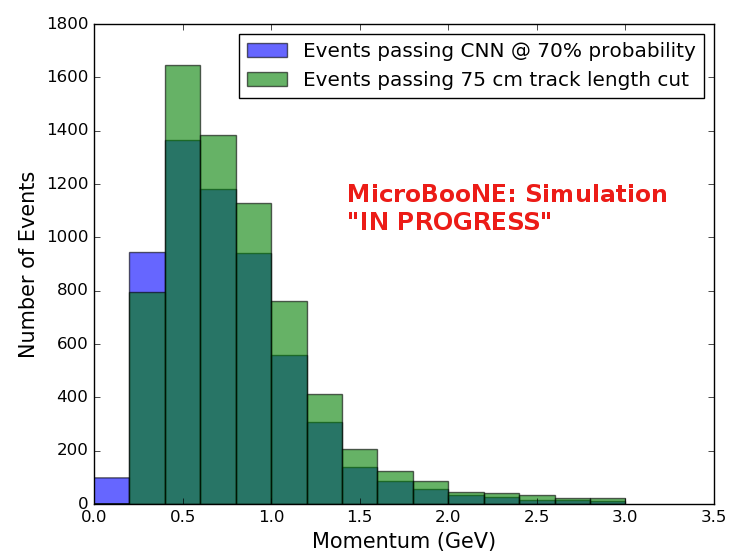
\includegraphics[width=3in,height=3in]{figs/sel1_parP_wrongnorm_acc70_0706.png}
	\caption{Momentum distribution of events from Selection I Original passing CNN with 70\% accuracy using image data with wrong normilazion}
	\label{fig:momentum_wrongnorm}
	\end{subfigure}
	\quad
	\begin{subfigure}[b]{.45\textwidth}
	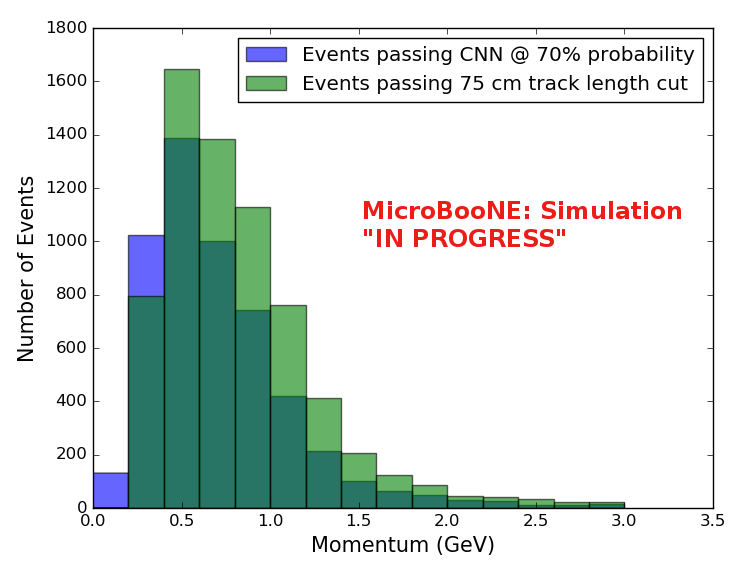
\includegraphics[width=3in,height=3in]{figs/sel1_parP_rightnorm_acc70_0706.png}
	\caption{Momentum distribution of events from Selection I Original passing CNN with 70\% accuracy using image data with correct normilazion}
	\label{fig:momentum_rightnorm}
	\end{subfigure}
	\quad
\caption{CNN10000 distributions of track candidate images output from Selection I Original cc-inclusive filter with different image data normalizations}
\label{fig:CNN_dist}
\end{figure}

The next step that was taken was to use CNN10000 to classify track candidate images that were identified by the selection I original cc-inclusive filter described in \cite{cc-inclusive}. Passing rates for each cut in cc-inclusive filter are show in figure \ref{fig:cuttable}. For the incorrect image making normalization dataset, out of 188,880 events, 7438 passed the cut right before 75 cm track length cut which is 3.9\% of total data. Discrepancies in passing rates are due to grid submission issues, however, this dataset is used to check if changes in image making normalization affects $\mu/\pi$ separation probability due to CNN10000 being trained with incorrectly image making normalized data. For the second dataset with correct image making normalization, out of 188,880 events, 9552 events passed the cut right before the 75 cm track length cut which is 5.1\% passing rate and is comparable to figure \ref{fig:cuttable}. In time cosmics were also run over for efficiency and purity calculations. Out of 14395 in time cosmic events, 175 passed the cut right before the 75 cm track length cut which is a passing rate of 1.2\% compared to 1.3\% shown in figure \ref{fig:cuttable}. 

Figures \ref{fig:confusion_wrongnorm}, \ref{fig:prob_wrongnorm}, \ref{fig:confusion_rightnorm} and \ref{fig:prob_rightnorm} show the accuracy and $\mu/\pi$ separation of both the correct and incorrect normalized images. The confusion matrices are only composed of $\mu/\pi$ data. Other particles passed the cc-inclusive filter before the 75 cm track length cut and were all mis-id'ed as muons. Since CNN10000 has not seen any particles other than muons and pions, it makes sense that those get mis-id'ed. Figures \ref{fig:prob_wrongnorm} and \ref{fig:prob_rightnorm} don't have $\mu/\pi$separation comparable to \ref{fig:prob_plot}, but \ref{fig:prob_wrongnorm} does skew to higher probabilities compared to \ref{fig:prob_rightnorm}. This is to be expected and further work on quantifying the performance of CNN10000 should use the incorrect image making normalization. It is also expected that the separation isn't as defined as the testing dataset for CNN10000. CNN10000 was trained and tested using single particle muons and pions and the track candidate dataset come from BNB+Cosmic events, not to mentions all track candidates have passed the cc-inclusive filter that tags "muon-like" tracks therefore the pions in this sample look much closer in muon topology than the network has seen. Also, these images were made from wire and time ticks associated to hits from the track candidate that passed the cc-inclusive filter. This is different from the training images where a bounding box was drawn over the total $\mu$ or $\pi$ interaction. Spurious energy deposition from a $\pi-Ar$ interaction is most likely not included in the BNB+Cosmic images due to the tracking algorithm. To remedy this, the neural network needs to see more "muon-like" pions and muons and pions from a neutrino interaction passing the cc-inclusive filter as well as a larger particle variety including protons, photons and electrons. Although $\mu/\pi$ separation is lacking, CNN10000 does an excellent job of classifying muons and using higher CNN probability can increase purity. Figures \ref{fig:track_wrongnorm}, \ref{fig:track_rightnorm}, \ref{fig:momentum_wrongnorm} and \ref{fig:momentum_rightnorm} show the track and momentum distributions for these two datasets. In both sets you have an increase in data in the bin below 75 cm and at bins below 0.5 GeV. These distributions were made with events classified with 70\% probability of being a muon regardless of true particle type. 

\section{Classification of MC data using Selection I Modified CC-Inclusive Filter}

\begin{figure}[htp!]
\centering
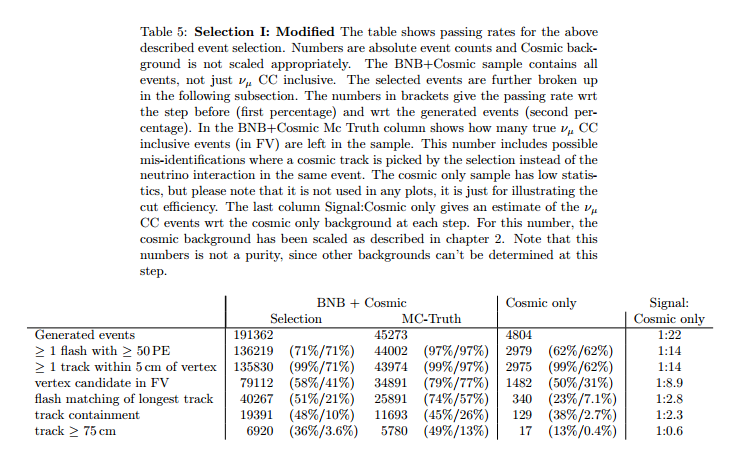
\includegraphics[width=.8\textwidth]{figs/cuttable_sel1mod.png}
\caption{Snapshot of passing rates of all cuts from Selection I Modified cc-inclusive filter}
\label{fig:table1}
\end{figure}

CNN10000 was also used to classify track candidate images that were identified by the selection I modified cc-inclusive filter described in \cite{cc-inclusive}. Passing rates for each cut in this filter are shown in figure \ref{fig:table1}. As seen in section \ref{sel1orig}, wrong image normalization had a higher muon classification probability so all work done using selection I modified cc-inclusive filter was done using this normalization. Out of 188,880 events, 19,112 passed the cut right before the 75 cm track length cut which is a 10.1\% passing rate and comparable to the 10\% passing rate shown in figure \ref{fig:table1}. In time cosmics were also run over, out of 14,606 in time cosmics events, 302 passed the cut right before the 75 cm track length cut which is a 2.1\% passing rate comparable to the 2.7\% passing rate in the cc-inclusive tech-note. Figures \ref{fig:confusion_sel1mod} and \ref{fig:prob_sel1mod} show the accuracy and $\mu/\pi$ separation. Both plots are only composed of muons and pions and like selection I original data, all other particles were id'ed as muons. Also like selection I original data, muons are being identified at a very high rate. 
Figure \ref{fig:sel1mod_track} shows the track range distributions of all events from selection I modified being classified by the CNN as a muon with a probability of 70\% regardless of true particle type. We get entries for the CNN curve in the lowest bin and none for the 75 cm curve. To see how many true CC events were identified by CNN10000 breaking down figure \ref{fig:sel1mod_track} by event type was necessary. Figures \ref{fig:sel1mod_stackedcnn} and \ref{fig:sel1mod_stackedoriginal} show track range distributions separated by signal and various backgrounds. Particle type was not taken into consideration in these plots so true CC event images can be any track candidate particle passing selection I modified cut right before track length cut including pions and protons. 

To gain an even deeper understanding on how CNN10000 is performing, plotting these distributions with only muons and pions was done due to the fact that CNN10000 was trained with only those particles for $\mu/\pi$ separation. Figures \ref{fig:sel1mod_mupi_70stackedcnn}-\ref{fig:sel1mod_mupi_90stackedcnn} show the stacked histograms of signal and background of the track range distributions with varying CNN probabilities starting from 70\% and ending at 90\% probability. With higher probabilities we get a purer sample in the lower bin but we end up losing events as well. Momentum distributions for all signal/background events are shown in figure \ref{fig:sel1mod_parP}.    

\begin{figure}[htp!]
\centering
	\begin{subfigure}[b]{.45\textwidth}
	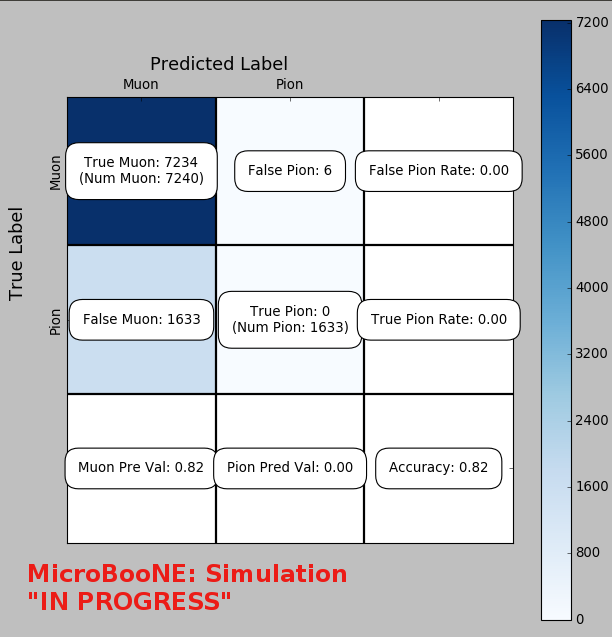
\includegraphics[width=3in,height=3in]{figs/sel1mod_confusion_wrongnorm.png}
	\caption{Confusion Matrix for CNN10000 classified events from selection I modified}
	\label{fig:confusion_sel1mod}
	\end{subfigure}
	\quad
	\begin{subfigure}[b]{.45\textwidth}
	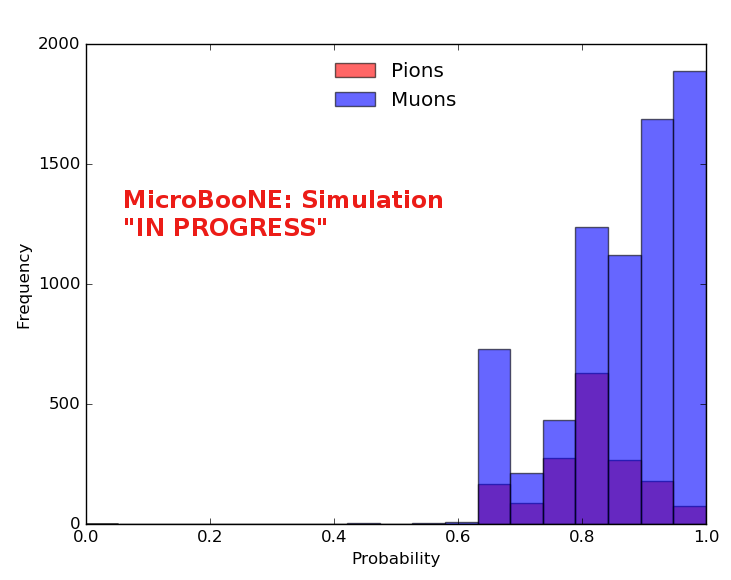
\includegraphics[width=3in,height=3in]{figs/probplot_wrongnorm_selImod.png}
	\caption{Probability plot for CNN10000 classified events from selection I modified}  
	\label{fig:prob_sel1mod}
	\end{subfigure}
	\quad
\caption{Confusion matrix and probability plot of events passing selection I modified cc-inclusive cuts right before 75cm track length cut}
\label{probplots}
\end{figure}

\begin{figure}[htp!]
\centering
	\begin{subfigure}[b]{.9\textwidth}
	\centering
	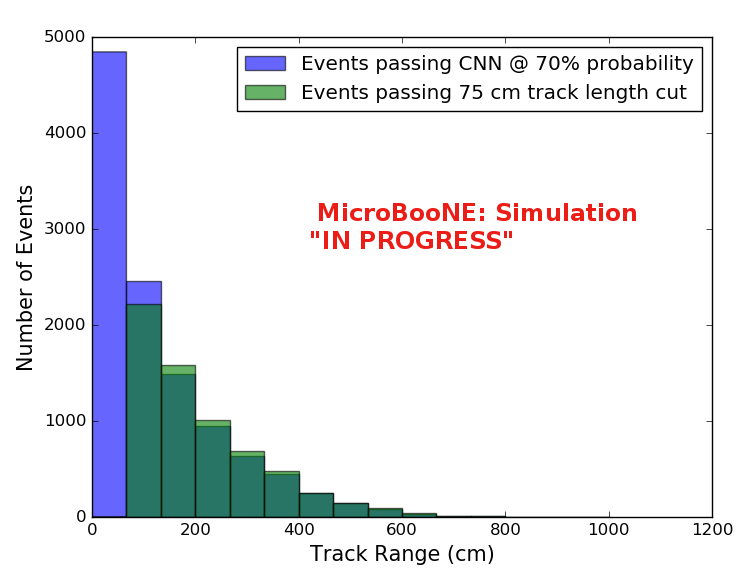
\includegraphics[width=4in,height=2.5in]{figs/sel1mod_trackrange_wrongnorm_acc70_0706.png}
	\caption{Track range distribution of events from Selection I Modified passing CNN with 70\% accuracy}
	\label{fig:sel1mod_track}
	\end{subfigure}
	\quad
	\begin{subfigure}[b]{.45\textwidth}
	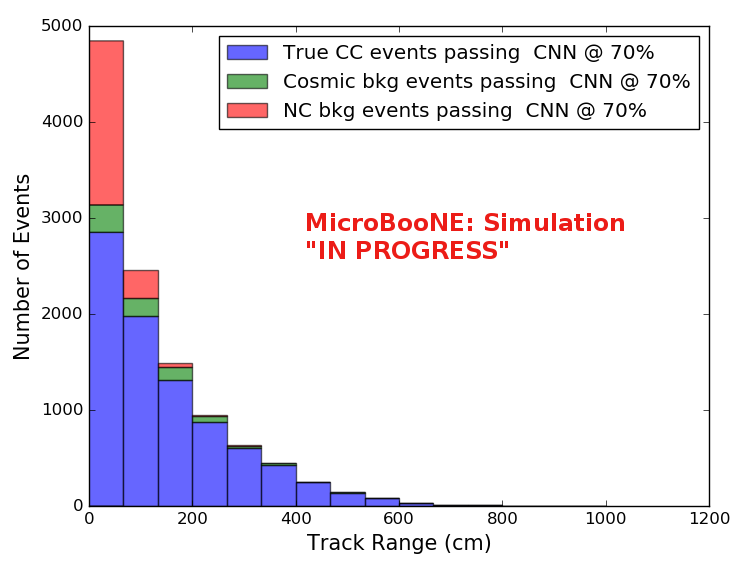
\includegraphics[width=\textwidth, height=2in]{figs/sel1mod_cnn_stackedevent_0707.png}
	\caption{Stacked signal and background track range distributions from Selection I Modified passing CNN with 70\% accuracy}
	\label{fig:sel1mod_stackedcnn}
	\end{subfigure}
	\quad
	\begin{subfigure}[b]{.45\textwidth}
	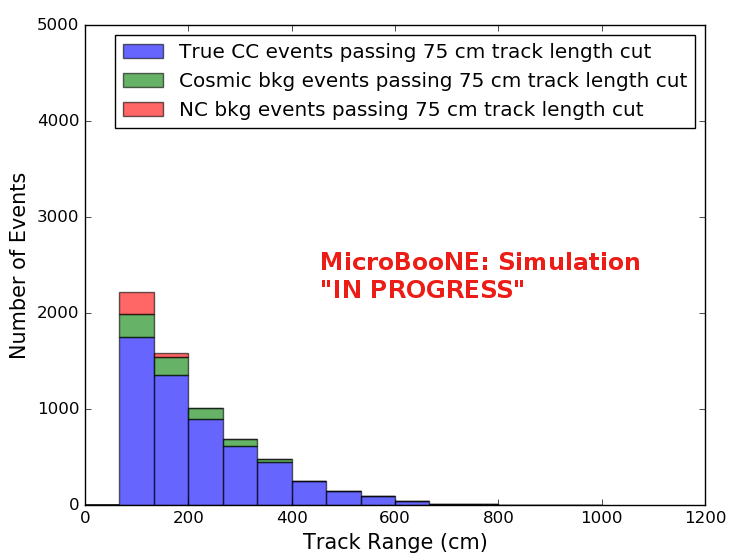
\includegraphics[width=\textwidth, height=2in]{figs/sel1mod_original_stackedevents_0707.png}
	\caption{Stacked signal and background track range distributions from Selection I Modified passing 75 cm track length cut}
	\label{fig:sel1mod_stackedoriginal}
	\end{subfigure}
	\quad
	\begin{subfigure}[b]{.45\textwidth}
	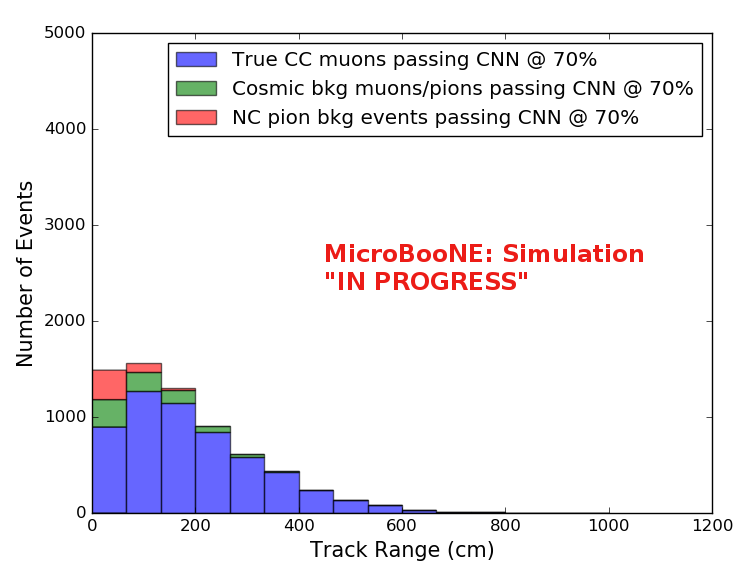
\includegraphics[width=\textwidth, height=2in]{figs/sel1mod_cnn_trackrange_mupi_acc70_0707.png}
	\caption{Stacked signal muons and background muons/pions of track range distributions from Selection I Modified passing CNN with 70\% accuracy}
	\label{fig:sel1mod_mupi_70stackedcnn}
	\end{subfigure}
	\quad
	\begin{subfigure}[b]{.45\textwidth}
	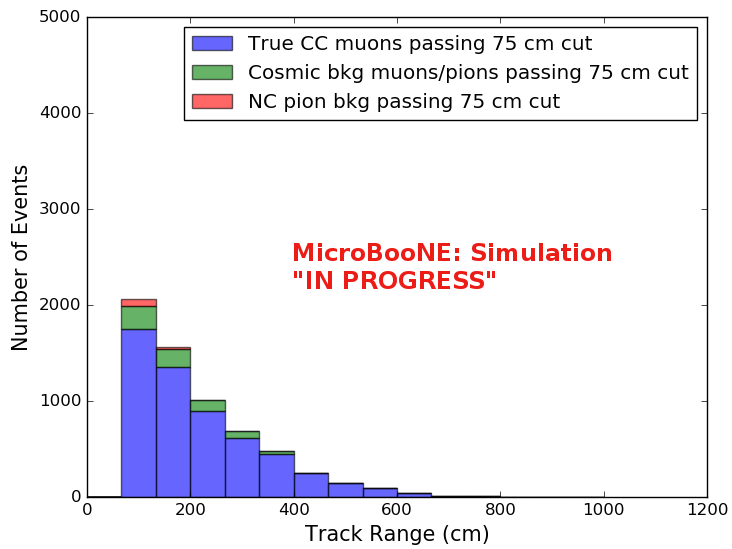
\includegraphics[width=\textwidth, height=2in]{figs/sel1mod_original_trackrange_mupi_acc70_0707.png}
	\caption{Stacked signal muons and background muons/pions of track range distributions from Selection I Modified passing 75 cm track length cut}
	\label{fig:sel1mod_mupi_70stackedoriginal}
	\end{subfigure}
	\quad
\caption{CNN10000 distributions of track candidate images output from Selection I Modified cc-inclusive filter}
\label{fig:sel1mod_CNN_dist}
\end{figure}



\begin{figure}[htp!]
\centering
	\begin{subfigure}[b]{.45\textwidth}
	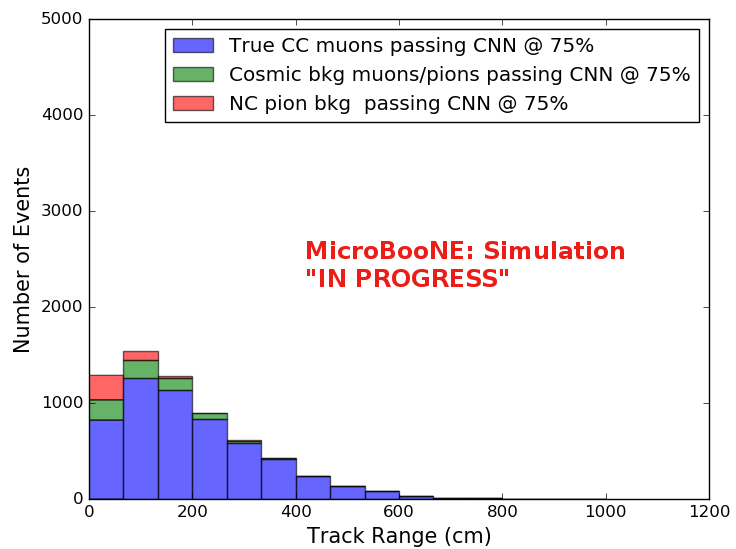
\includegraphics[width=\textwidth, height=2.5in]{figs/sel1mod_cnn_trackrange_acc75_0707.png}
	\caption{Stacked signal muons and background muons/pions of track range distributions from Selection I Modified passing CNN with 75\% accuracy}
	\label{fig:sel1mod_mupi_75stackedcnn}
	\end{subfigure}
	\quad
	\begin{subfigure}[b]{.45\textwidth}
	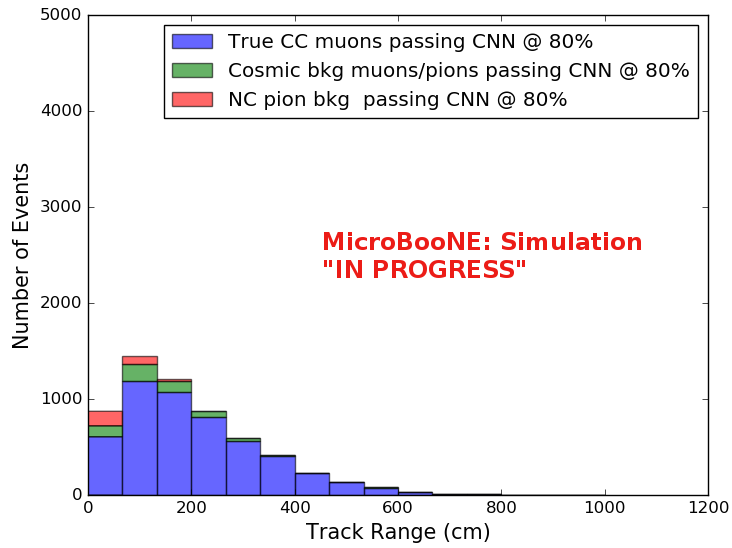
\includegraphics[width=\textwidth, height=2.5in]{figs/sel1mod_cnn_trackrange_acc80_0707.png}
	\caption{Stacked signal muons and background muons/pions of track range distributions from Selection I Modified passing CNN with 80\% accuracy}
	\label{fig:sel1mod_mupi_80stackedcnn}
	\end{subfigure}
	\quad
	\begin{subfigure}[b]{.45\textwidth}
	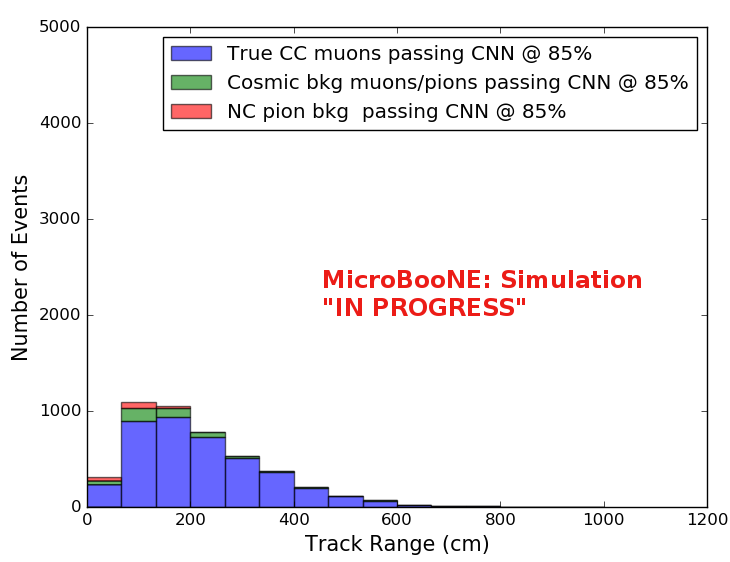
\includegraphics[width=\textwidth, height=2.5in]{figs/sel1mod_cnn_trackrange_acc85_0707.png}
	\caption{Stacked signal muons and background muons/pions of track range distributions from Selection I Modified passing CNN with 85\% accuracy}
	\label{fig:sel1mod_mupi_85stackedcnn}
	\end{subfigure}
	\quad
	\begin{subfigure}[b]{.45\textwidth}
	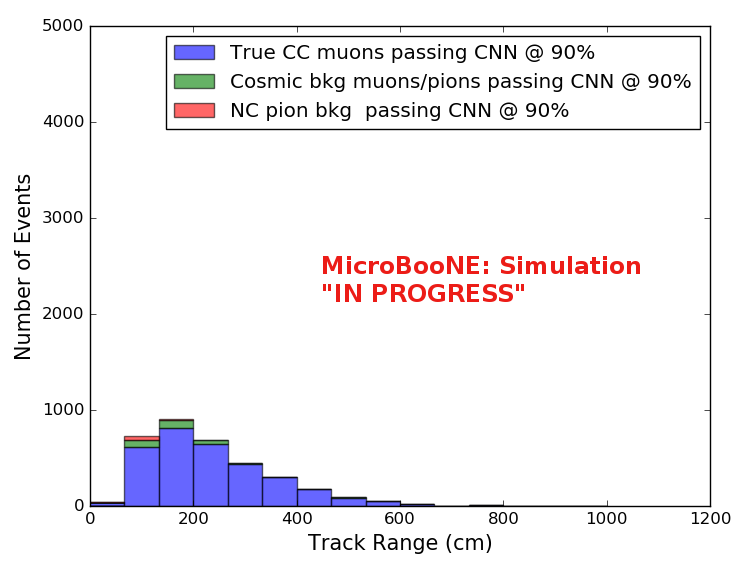
\includegraphics[width=\textwidth, height=2.5in]{figs/sel1mod_cnn_trackrange_acc90_0707.png}
	\caption{Stacked signal muons and background muons/pions of track range distributions from Selection I Modified passing CNN with 90\% accuracy}
	\label{fig:sel1mod_mupi_90stackedcnn}
	\end{subfigure}
	\quad
\caption{CNN10000 stacked signal/background track range distributions of track candidate images output from Selection I Modified cc-inclusive filter}
\label{fig:sel1modCNNdistacc}
\end{figure}


\begin{figure}[htp!]
\centering
	\begin{subfigure}[b]{.9\textwidth}
	\centering
	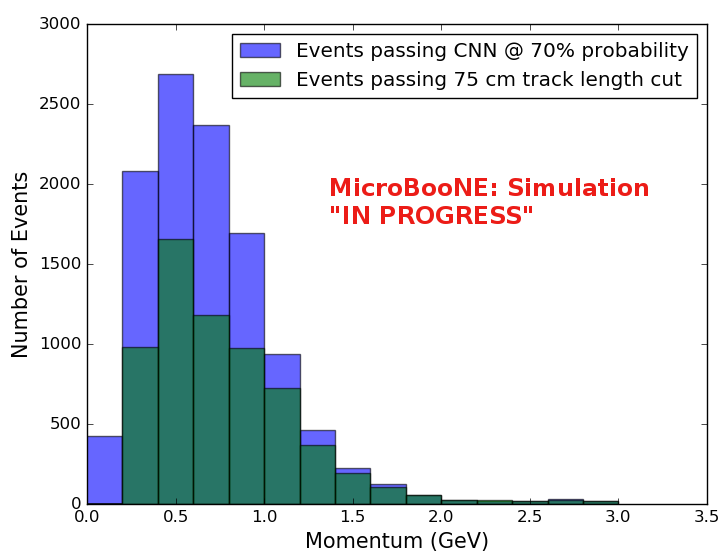
\includegraphics[width=\textwidth,height=3.5in]{figs/sel1mod_parP_wrongnorm_acc70_0706.png}
	\caption{Momentum distribution of events from Selection I Modified passing CNN with 70\% accuracy}
	\label{fig:sel1mod_momentum}
	\end{subfigure}
	\quad
	\begin{subfigure}[b]{.45\textwidth}
	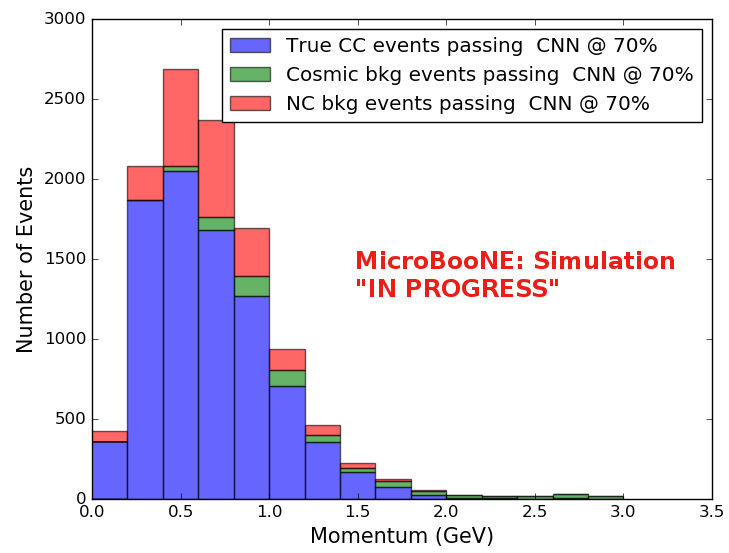
\includegraphics[width=\textwidth,height=2.5in]{figs/sel1mod_cnn_parP_stackedevents_0707.png}
	\caption{Stacked signal and background momentum distributions from Selection I Modified passing CNN with 70\% accuracy}
	\label{fig:sel1mod_momentum_stackedcnn}
	\end{subfigure}
	\quad
	\begin{subfigure}[b]{.45\textwidth}
	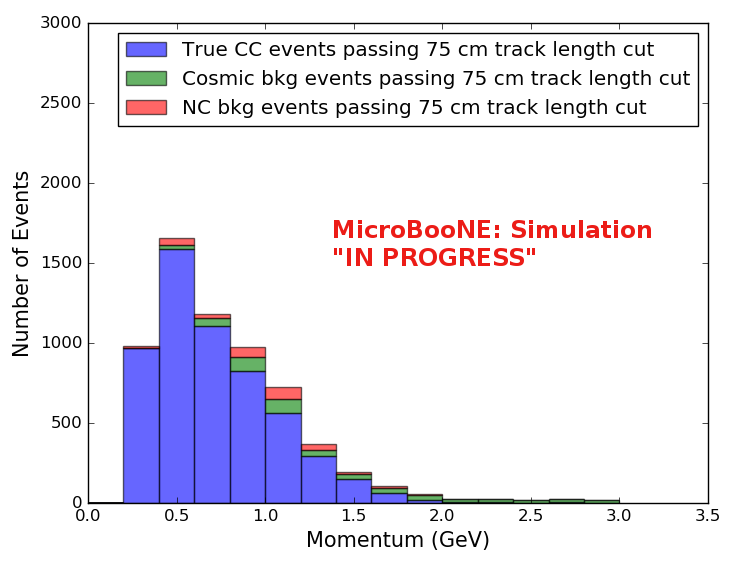
\includegraphics[width=\textwidth,height=2.5in]{figs/sel1mod_original_parP_stackedevents_0707.png}
	\caption{Stacked signal and background momentum distributions from Selection I Modified passing 75 cm track length cut}
	\label{fig:sel1mod_momentum_stackedoriginal}
	\end{subfigure}
	\quad
\caption{CNN10000 momentum distributions of track candidate images output from Selection I Modified cc-inclusive filter}
\label{fig:sel1mod_parP}
\end{figure}

Another check was to see if any true CC pions were passing through the cut right before the 75 cm track length cut. Figure \ref{fig:mupi} shows the comparison of the stacked track range distribution with only true CC muon signal versus the stacked distribution with true CC muons and pions signal. As you can see, we gain more events when plotting CC events with a particle type of either muons or pions due to the CNN classifying all pions in this dataset as muons. This is an interesting scenario and a sample of topologies of these images are represented in figure \ref{fig:evd}, at least 3 tracks are coming out of the vertex for these types of events. With the 75 cm track length cut, the selection is cutting event topologies like this where the pion is the tagged track candidate. Figure \ref{fig:longer_muon_badreco} has a defined longer muon track, but because of dead wires through the track, the reconstructed range is 1. less than 75 cm and 2. shorter than the reconstructed pion whose length is also less than 75 cm. This is a very interesting event, but because of issues with the tracking algorithm, the 75 cm cut would get rid of this event. The CNN was able to recover this event only because it has classified all pions as muons. Figure \ref{fig:longer_pion} shows the second case to think about, the pion, while still less than 75 cm has a reconstructed track length longer than the muon. Again, the CNN recovered this event due to pions being classified as muons. Lastly, figure \ref{fig:verylongpion} shows a pion with a reconstructed track length greater than 75 cm and the muon. These three cases show that a broader question must be asked when training the network other than is it a muon or pion. There are different routes to recover interesting events like these. One route is to ask the network ``Is it a CC event or is it an NC event?'' and obtain an image dataset consisting of whole CC/NC events that will train the network to answer this question. The other route is to ask the network ``Is this a $\mu/\pi/p/$ from a CC event or NC event and obtain an image dataset consisting of primary particles from a CC/NC event. Both these paths will be explored in future work.     

\begin{figure}[htp!]
\centering
	\begin{subfigure}[b]{.45\textwidth}
	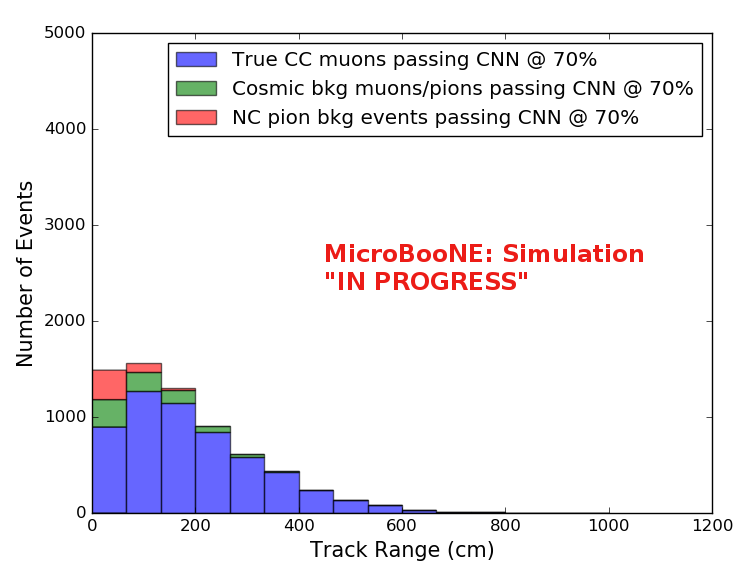
\includegraphics[width=\textwidth,height=2.5in]{figs/sel1mod_cnn_trackrange_mupi_acc70_0707.png}
	\caption{Stacked signal $\mu$/backround $\mu$ and $\pi$ track range distribution of CNN @ 70\%}
	\end{subfigure}
	\quad
	\begin{subfigure}[b]{.45\textwidth}
	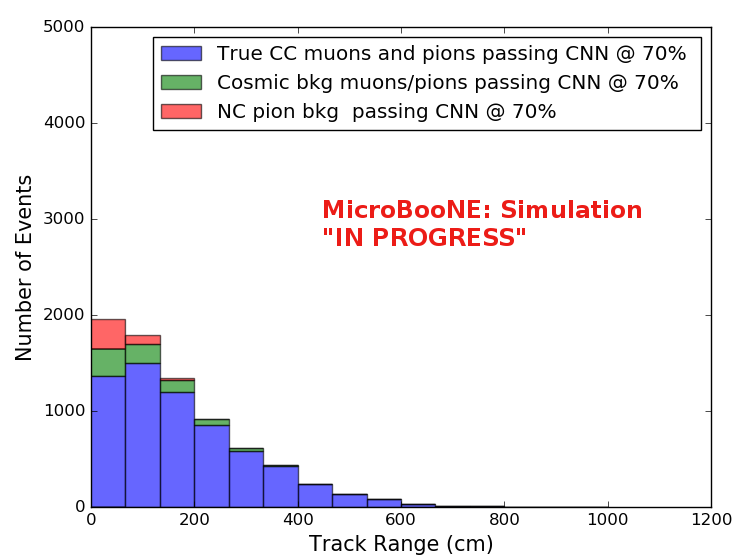
\includegraphics[width=\textwidth,height=2.5in]{figs/sel1mod_mupi_trackrange_acc70.png}
	\caption{Stacked signal $\mu \& \pi$/backround $\mu \& \pi$ track range distribution of CNN @ 70\%}
	\end{subfigure}
	\quad
\caption{Track distribution comparisons of true CC muons plotted vs true CC muons and pions plotted}
\label{fig:mupi}
\end{figure}


\begin{figure}[htp!]
\centering
	\begin{subfigure}[b]{.3\textwidth}
	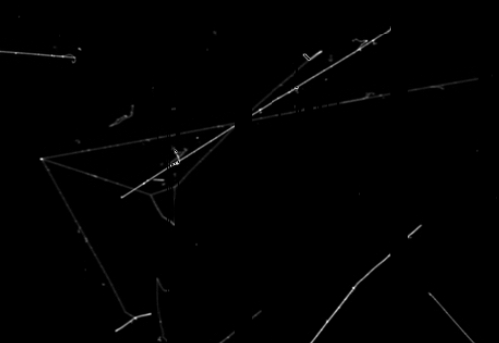
\includegraphics[width=\textwidth,height=2.5in]{figs/interesting_event.png}
	\caption{Pion recontructed track range is less than 75 cm and longer than muon reconstructed track due to dead wires}
	\label{fig:longer_muon_badreco}
	\end{subfigure}
	\quad
	\begin{subfigure}[b]{.3\textwidth}
	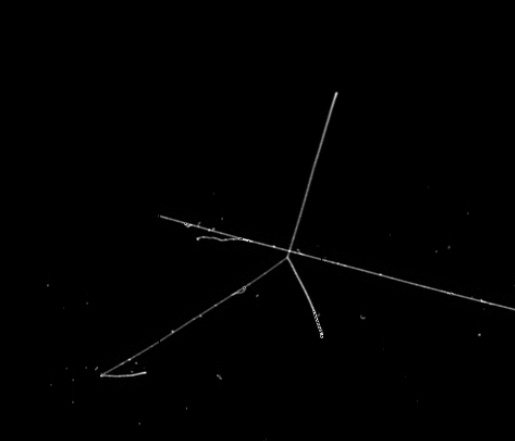
\includegraphics[width=\textwidth,height=2.5in]{figs/event2.png}
	\caption{Pion recontructed track range is less than 75 cm and larger than muon reconstructed track}
	\label{fig:longer_pion}
	\end{subfigure}
	\quad
	\begin{subfigure}[b]{.3\textwidth}
	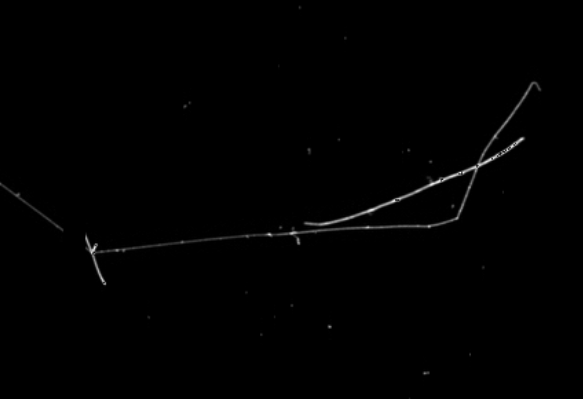
\includegraphics[width=\textwidth,height=2.5in]{figs/mupievent.png}
	\caption{Pion reconstructed track range is greater than 75 cm and larger than muon reconstructed track}
	\label{fig:verylongpion}
	\end{subfigure}
	\quad
\caption{Images of true CC events where the pion was the tagged track candidate}
\label{fig:evd}
\end{figure}

\pagebreak[4]
\pagebreak[4]
\pagebreak[4]

\begin{table}[htp!]
\centering
\resizebox{\textwidth}{!}{ \begin{tabular}{c||c| c c| c| c} % centered columns (4 columns)
\hline %inserts double horizontal lines
\toprule 
      && \multicolumn{2}{c}{BNB + Cosmics} & \multicolumn{1}{c}{Cosmic Only} & \multicolumn{1}{c}{Signal:}\\

      && Selection & MC Truth & &Cosmic Only \\

\midrule
75 cm Cut passing rates	& Generated Events  	       & 191362             & 45723               & 4804                & 1:22 \\ % inserting body of the table
                        & Track Containment 	       & 19391 (48\%/10\%)  & 11693 (45\%/26\%)   & 129 (38\%/2.7\%)    & 1:2.3  \\
\rowcolor{LightCyan}    & track $\geq$ 75 cm 	       & 6920 (36\%/3.6\%)  & 5780 (49\%/13\%)    & 17 (13\%/0.4\%)     & 1:0.6  \\
\hline\hline
CNN passing rates       & Generated Events  	       & 188880             & 44689               & 14606               & 1:21 \\ % inserting body of the table
		        & Track Containment 	       & 19112 ( /10\%)     & 11554 ( /26\%)      & 302 ( /2.1\%)       & 1:1.73  \\
\rowcolor{LightCyan}    & CNN cut @ 70\% Probability   & 16502 (86\%/8.7\%) & 10605 (92\%/23\%)   & 205 (68\%/14\%)     & 1:1.28  \\
\rowcolor{LightCyan}    & CNN cut @ 83\% Probability   & 7511 (46\%/4.0\%)  & 6142  (58\%/14\%)   & 32 (16\%/0.2\%)     & 1:0.4  \\
\bottomrule
\hline %inserts single line
\end{tabular}}
\caption{Comparing passing rates of CNN at different probabilities versus 75 cm track length cut: Numbers are absolute event counts and Cosmic background is not scaled appropriately. The BNB+Cosmic sample contains all events. The numbers in brackets give the passing rate wrt the step before (first percentage) and wrt the generated events (second percentage). In the BNB+Cosmic MC Truth column shows how many true $\nu_{\mu}$ CC-inclusive events (in FV) are left in the sample. This number includes possible mis-identifications where a cosmic track is picked by the selection instead of the neutrino interaction in the same event.The CNN MC True generated events were scaled wrt the MC True generated events for the 75 cm cut passing rates due to only running over 188,880 generated events versus the 191362 generated events. The last column Signal:Cosmic only gives an estimate of the $\nu_{\mu}$ CC events wrt the cosmic only background at each step. For this number, the cosmic background has been scaled as described in \cite{cc-inclusive}. Note that these numbers are not a purity, since other backgrounds can’t be determined at this step.} 
% title of Table
\label{table:passingrates} % is used to refer this table in the text
\end{table}


\begin{table}[htp!]
\centering
\resizebox{\textwidth}{!}{ \begin{tabular}{c c c|a} % centered columns (4 columns)
%\hline %inserts double horizontal lines
      &&\#Events(Fraction)  & \#Events(Fraction) \\
      &&passing CNN @ 70\% Probability & passing CNN @ 83\% Probability\\


Signal	       & $\nu_{\mu}$ CC events with true vertex in FV      & 10605(35\%)       & 6142(61\%)\\ % inserting body of the table
\hline\hline %inserts double horizontal lines
Backgrounds    & Cosmics Only Events                               & 13573(45\%)       & 2582(26\%)\\ % inserting body of the table
               & Cosmics in BNB Events                             & 2249(7.4\%)       & 492(4.9\%)\\ % inserting body of the table
               & NC Events                                         & 3412(11\%)        & 778(7.7\%)\\ % inserting body of the table
               & $\nu_e$ and $\bar{\nu}_e$ Events                  & 139(0.5\%)        & 32(0.3\%)\\ % inserting body of the table
               & $\bar{\nu}_{\mu}$  Events                         & 97(0.3\%)         & 67(0.7\%)\\ % inserting body of the table
\end{tabular}}
\caption{Signal and background event numbers at modified selection level with CNN cut estimated from a BNB+Cosmic sample and Cosmic only sample normalized to $5*10^{19}$ PoT. The last column gives the fraction of this signal or background type to the total selected events per CNN probability.} 
\label{table:purity} % is used to refer this table in the text
\end{table}

Table \ref{table:passingrates} shows the passing rates for the 75 cm track length cut and the CNN cut at 70\% and 83\%. The passing rates at the track containment level for the 75 cm track length cut compared to the CNN are comparable with only a 0.6\% difference in the in time cosmic bin which may be due in part to the larger in time cosmic statistics used for the CNN dataset. These passing rates need to be comparable to then be able to compare the passing rates after the CNN cut to the 75 cm cut. Again, the same BNB+Cosmic sample was used for both selection I modified with 75 cm cut and selection I modified with CNN cut. As it stands, a CNN cut at 83\% probability has a MC true CC event passing rate of 14\% compared to the 13\% passing rate of the 75 cm track length cut. The Signal:Cosmic Only background is also reduced from 1:0.6 to 1:0.4 The total passing rate is also higher than the 75 cm cut, 3.6\% vs 4.0\%. Table \ref{table:purity} shows the breakdown of signal and backgrounds for the CNN at the different probabilities. We have a 61\% signal passing rate with the CNN cut @ 83\% versus the 53.8\% signal passing rate of the 75 cm cut. 

Based on these numbers, the following performance values of the modified selection with 75 cm cut versus modified selection with CNN @ 83\% probability cut were calculated:
\begin{itemize}
\item Efficiency: Number of selected true $\nu_{\mu}$ CC events divided by the number of expected true $\nu_{\mu}$ CC events with interaction in the FV.
\begin{itemize}
\item Selection I modified: 13\% 
\item Selection I modified with CNN cut @ 83\% probability: 14\% 
\end{itemize}
\item Purity: Number of selected true $\nu_{\mu}$ CC events divided by sum of itself and the number of all backgrounds.
\begin{itemize}
\item Selection I modified: 53.8\% 
\item Selection I modified with CNN cut @ 83\% probability: 61\% 
\end{itemize}
\end{itemize}

Lastly, figure \ref{fig:sel1mod_cnnperformance} shows a more representative performance of the CNN. Due to the fact that the CNN was trained on muons and pions, showing the performance of CC muon events versus NC pion events with respect to CNN probability gives a better picture of how the network is performing. Figure \ref{fig:sel1mod_cnnperformance} shows that at 83\% we are below the 75 cm cut NC pion threshold and still above the CC muon threshold. Using 83\% probability not only reduced the NC pion background, it also dramatically reduced the in time cosmics and cosmics in the BNB. 

\begin{figure}[htp!]
\centering
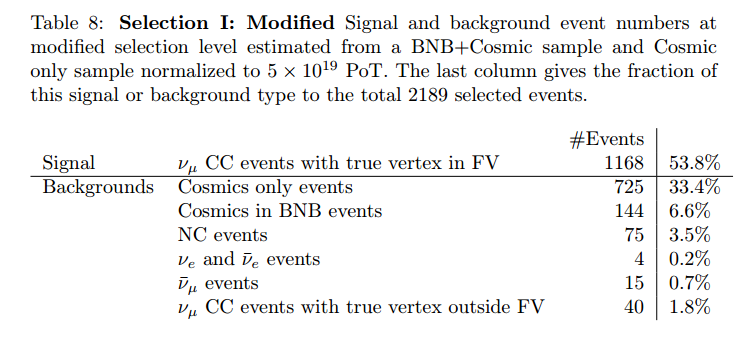
\includegraphics[width=4in,height=2.5in]{figs/purity_sel1mod.png}
\caption{Snapshot of signal and background event numbers of Selection I modified from cc-inclusive note \cite{cc-inclusive}}
\label{fig:pur_sel1mod}
\end{figure}

\begin{figure}[htp!]
\centering
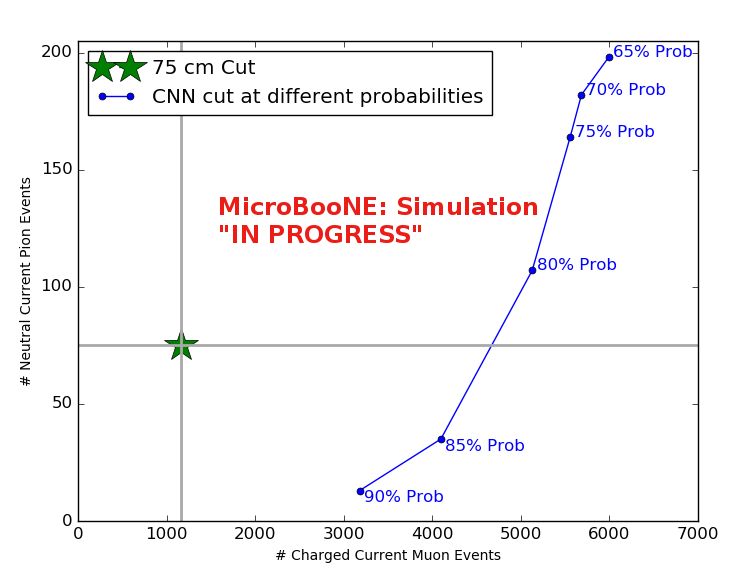
\includegraphics[width=3in,height=2.5in]{figs/cnn_performance.png}
\caption{CNN performance of classified muons and pions compared to the already implemented 75 cm track length cut}
\label{fig:sel1mod_cnnperformance}
\end{figure}

\section{Conclusions and Future Work}

It was shown that even though CNN10000 was trained with single particle generated muons and pions, it performs fairly well at classifying track candidate images from BNB+Cosmic events. Events have been regained below the 75 cm track length cut and the momentum and track range distributions have similar shapes to the distributions of Selection I original and modified. Efficiencies and purities were calculated for selection I modified events before 75 cm track length cut  with the CNN at 83\% probability and are 14\% and 62\% respectively. Although the CNN doesn't have separation between muons and pions and although all particles passing CNN are classified as muon, increasing CNN probability allows us to increase the purity as well as maintain an efficiency comparable to the 75 cm track length cut all while recovering events below that 75 cm cut. Out of the 6142 events that passed the CNN @ 83\% 1470 events were below the 75 cm cut, a recovery of 3.3\% of data with an purity of 15\%. Although these numbers are low, it is an improvement from the selecion I modified in both total efficiency and purity and an increase in phase space by recovering these events. The next steps are to train two additional neural networks. One with track candidate muon and pion images originating from BNB+Cosmic events and the second whole $CC_{\mu}/NC_{\pi}$ events to gauge CNN performance. These trainings are underway.

\clearpage

